\documentclass[12pt, a4paper]{article}
\usepackage[utf8]{inputenc}
\usepackage{amsmath}
\usepackage{amsthm}
\usepackage{amssymb}
\usepackage{graphicx}
\usepackage{parskip}
\usepackage{hyperref}
\usepackage{fancyhdr}
\usepackage{lastpage}
\usepackage[vlined,ruled]{algorithm2e}
\usepackage[acronym]{glossaries}
\usepackage{caption}
\usepackage{titlesec}
\usepackage{tikz}
\usetikzlibrary{arrows,automata}

\titleformat{\section}
  {\normalfont\bfseries}{Problem 8.\thesection}
  {0em}{}

\titleformat{\subsection}
  {\normalfont\bfseries}{8.\thesubsection}
  {0em}{}

\titleformat{\subsubsection}
  {\normalfont\bfseries}{8.\thesubsection}
  {0em}{}

\title{%
  Stochastic Network Modeling \\
  Homework 8 - Solutions
}
\author{%
  Juan Pablo Royo Sales\\
  \small{Universitat Politècnica de Catalunya}
}
\date\today

\pagestyle{fancy}
\fancyhf{}
\fancyhead[C]{}
\fancyhead[R]{Juan Pablo Royo Sales - UPC MIRI}
\fancyhead[L]{SNM - Homework 8}
\fancyfoot[L,C]{}
\fancyfoot[R]{Page \thepage{} of \pageref{LastPage}}
\setlength{\headheight}{15pt}
\renewcommand{\headrulewidth}{0.4pt}
\renewcommand{\footrulewidth}{0.4pt}

\renewcommand{\qedsymbol}{$\blacksquare$}

\begin{document}

\maketitle

\section{}
\subsection{}
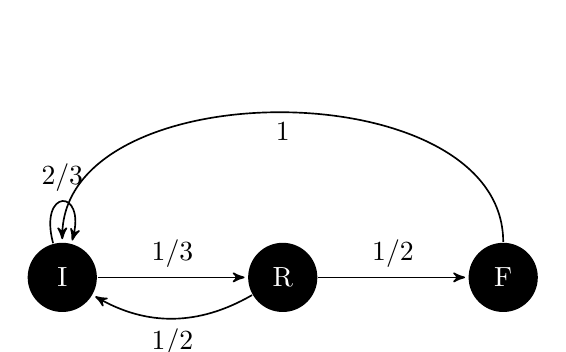
\begin{tikzpicture}[->,>=stealth',shorten >=1pt,auto,node distance=2.8cm,
  semithick]
  \tikzstyle{every state}=[fill=black,draw=none,text=white]

  \node[state]         (A)              {I};
  \node[state]         (B) [right of=A] {R};
  \node[state]         (C) [right of=B] {F};

  \path (A) edge              node {1/3} (B)
        (A) edge [loop above] node {2/3} (A)
        (B) edge [bend left]  node {1/2} (A)
        (B) edge              node {1/2} (C)
        (C) edge [bend right=90] node {1} (A)
        ;
\end{tikzpicture}

\begin{align*}
  P = \begin{bmatrix}
       & I & R & F\\
     I & 2/3 & 1/3 & 0\\
     R & 1/2 & 0 & 1/2 \\
     F & 1 & 0 & 0 \\
\end{bmatrix}
\end{align*}

\subsection{}

\begin{subequations}
  \begin{align}
    \begin{cases} 
      \pi_I \frac{1}{3} &= \pi_R \frac{1}{2} \implies \pi_I \frac{2}{3} = \pi_R\\
      \pi_I \frac{1}{3} &= \pi_F\\
      \sum \pi_i = 1
    \end{cases}
  \end{align}
\end{subequations}

\begin{subequations}
  \begin{align}
    \pi_I &= \frac{1}{1+\frac{2}{3}+\frac{1}{3}} = \frac{1}{2}\\
  \end{align}
\end{subequations}

Therefore $\pi_I = \frac{1}{2}, \pi_R = \frac{1}{3}, \pi_F = \frac{1}{6}$
\subsection{}
$S = p \times \pi_F = \frac{1}{3} \times \frac{1}{6} = \frac{1}{18}$
\subsection{}
$\begin{cases}
  1 & \text{ if it reaches to the end } \pi_F\\
  0 & \text{ otherwise }
\end{cases}$

\begin{subequations}
  \begin{align}
    E[T] &= \sum_{i=0}^n \pi_F \\
         &= \sum_{i=0}^n \frac{1}{6}\\
         &= \frac{n}{6}
  \end{align}
\end{subequations}

\section{}
\subsection{}
\begin{subequations}
  \begin{align}
    \begin{cases} 
      \pi_a &= \pi_b \alpha\\
      \pi_b (1-\alpha) &= \pi_c\\
      \sum \pi_i = 1
    \end{cases}
  \end{align}
\end{subequations}

\begin{subequations}
  \begin{align}
    \pi_b &= \frac{1}{1+\alpha+(1-\alpha)} = \frac{1}{2}\\
  \end{align}
\end{subequations}

Therefore $\pi_a = \frac{\alpha}{2}, \pi_b = \frac{1}{2}, \pi_c = \frac{1-\alpha}{2}$

\subsection{}
\subsection{}
$S = \pi_a = \frac{\alpha}{2}$
\subsection{}
$E[T] = \frac{1}{\pi_a} = 2$

\section{}
Lets the probabilities according to the definition be:
\begin{itemize}
  \item $p_{ab} = \frac{1}{3}$
  \item $p_{ac} = \frac{1}{3}$
  \item $p_{ad} = \frac{1}{3}$
  \item $p_{ba} = 1$
  \item $p_{db} = 1$
  \item $p_{ca} = \frac{1}{2}$
  \item $p_{cd} = \frac{1}{2}$
\end{itemize}

Solving by flux method

\begin{subequations}
  \begin{align}
    \begin{cases} 
      \pi_a \frac{1}{3} &= \pi_b\\
      \pi_a \frac{1}{3} &= \pi_c \frac{1}{2} \implies \pi_a \frac{2}{3} = \pi_c\\
      \pi_a \frac{1}{3} &= \pi_d\\
      \sum \pi_i = 1
    \end{cases}
  \end{align}
\end{subequations}

\begin{subequations}
  \begin{align}
    \pi_a &= \frac{1}{1+\frac{1}{3}+\frac{2}{3}+\frac{1}{3}}\\
          &= \frac{3}{7}
  \end{align}
\end{subequations}

Therefore $\pi_a = \frac{3}{7}, \pi_b = \pi_d = \frac{1}{7}, \pi_c = \frac{2}{7}$

\end{document}

